\documentclass[12pt]{article}

\usepackage{cmap}
\usepackage[T2A]{fontenc}
\usepackage[utf8]{inputenc}
\usepackage[russian]{babel}
\usepackage{graphicx}
\usepackage{amsthm,amsmath,amssymb}
\usepackage{listings}
\usepackage{color}
\usepackage[table]{xcolor}
\usepackage{colortbl}
\usepackage{array}
\usepackage{epigraph}
\usepackage{textcomp}

\usepackage[russian,colorlinks=true,urlcolor=red,linkcolor=blue]{hyperref}
\usepackage{enumerate}
\usepackage[shortlabels]{enumitem}
\usepackage{datetime}
\usepackage{fancyhdr}
\usepackage{lastpage}
\usepackage{verbatim}
\usepackage{tikz}
\usetikzlibrary{arrows,patterns,decorations.markings,decorations.pathmorphing,decorations.pathreplacing}
\usetikzlibrary{math,positioning}
\usepackage{pgfplots}

\usepackage{ifthen}
\usepackage{mathtools}
\usepackage{mdframed}
\usepackage[normalem]{ulem}

\graphicspath{ {notes-13-adversarial} }

\def\SEASON{2024/25}


\sloppy
\voffset=-20mm
\textheight=235mm
\hoffset=-22mm
\textwidth=180mm
\headsep=12pt
\footskip=20pt

\parskip=0em
\parindent=0em

\setlength\epigraphwidth{.8\textwidth}

\newlength{\tmplen}
\newlength{\tmpwidth}
\newlength{\storelen}
\newcounter{listcounter}

% Список с маленькими отступами
\newenvironment{MyList}[1][4pt]{
  \begin{enumerate}[1.]
  \setlength{\parskip}{0pt}
  \setlength{\itemsep}{#1}
}{       
  \end{enumerate}
}
% Вложенный список с маленькими отступами
\newenvironment{InnerMyList}[1][0pt]{
  \vspace*{-0.5em}
  \begin{enumerate}[(a)]
  \setlength{\parskip}{-0pt}
  \setlength{\itemsep}{#1}
}{       
  \end{enumerate}
  \vspace*{-0.5em}
}
% Список с маленькими отступами
\newenvironment{MyItemize}[1][4pt]{
  \begin{itemize}
  \setlength{\parskip}{0pt}
  \setlength{\itemsep}{#1}
}{       
  \end{itemize}
}

% Основные математические символы
\def\TODO{{\color{red}\bf TODO}}
\def\N{\mathbb{N}}       %
\def\R{\mathbb{R}}       %
\def\F2{\mathbb{F}_2}    %
\def\Z{\mathbb{Z}}       %
\def\H{\mathcal{H}}      % семество хеш-функций
\def\E{\mathsf{E}}       % матожидание
\def\INF{\infty}    % +inf
\def\EPS{\varepsilon}    %
\def\EMPTY{\varnothing}  %
\def\PHI{\varphi}        %
\def\SO{\Rightarrow}     % =>
\def\EQ{\Leftrightarrow} % <=>
\def\t{\texttt}          % mono font
\def\c#1{{\rm\sc{#1}}}   % font for classes NP, SAT, etc
\def\O{\mathcal{O}}      %
\def\NO{\t{\#}}          % #
\def\XOR{\text{ {\raisebox{-2pt}{\ensuremath{\Hat{}}}} }}
\def\xor{\t{\^{}}}
\renewcommand{\le}{\leqslant}
\renewcommand{\ge}{\geqslant}
\newcommand{\q}[1]{\langle #1 \rangle}               % <x>
\newcommand\URL[1]{{\footnotesize{\url{#1}}}}        %
\newcommand{\sfrac}[2]{{\scriptstyle\frac{#1}{#2}}}  % Очень маленькая дробь
\newcommand{\mfrac}[2]{{\textstyle\frac{#1}{#2}}}    % Небольшая дробь
\newcommand{\score}[1]{{\bf\color{red}{(#1)}}}
\newcommand{\divby}{\mathop{\raisebox{-2pt}{\vdots}}}

\newcommand{\fix}[1]{{\color{fixcolor}{#1}}} % \underline
\def\bonus{\t{\red{(*)}}}
\def\ifbonus#1{\ifthenelse{\equal{#1}{}}{}{\bonus}}
\def\smallsquare{$\scalebox{0.5}{$\square$}$}
\def\vstick{^\t{\textquotesingle}}
\def\bluebox#1{\fcolorbox{blue}{white}{#1}}

\newlength{\myItemLength}
\setlength{\myItemLength}{0.3em}
\def\ItemSymbol{\smallsquare}
\def\Item{\vspace*{\myItemLength}\ItemSymbol \ \ }

\newcommand{\LET}{%
  % [line width=0.6pt]
  \begin{tikzpicture}%
  \draw(0.8ex,0) -- (0.8ex,1.6ex);%
  \draw(0,1.6ex) -- (0.8ex,1.6ex);%
  \end{tikzpicture}%
  \hspace*{0.1em}%
}

% Отступы
\def\makeparindent{\hspace*{\parindent}\unskip}
\def\up{\vspace*{-0.5em}}%{\vspace*{-\baselineskip}}
\def\down{\vspace*{0.5em}}
\def\LINE{\vspace*{-1em}\noindent \underline{\hbox to 1\textwidth{{ } \hfil{ } \hfil{ } }}}
\def\BOX#1{\mbox{\fbox{\bf{#1}}}}
\def\Pagebreak{\pagebreak\vspace*{-1.5em}}
\def\RIGHT{\hspace*{\fill}} % сдвинуться до упора вправо
\def\NewLine{\hspace*{1em}\\}

% Мелкий заголовок
\newcommand{\THEE}[1]{
  \vspace*{0.5em}
  \noindent{\bf \underline{#1}}%\hspace{0.5em}
  \vspace*{0.2em}
}
% Другой тип мелкого заголовка
\newcommand{\THE}[1]{
  \vspace*{0.5em} $\bullet$
  \noindent{\bf #1}%\hspace{0.5em}
  \vspace*{0.2em}
}

\newenvironment{MyTabbing}{
  \t\bgroup
  \vspace*{-\baselineskip}
  \begin{tabbing}
    aaaa\=aaaa\=aaaa\=aaaa\=aaaa\=aaaa\kill
}{
  \end{tabbing}
  \t\egroup
}

% Код с правильными отступами
\lstnewenvironment{code}{
  \lstset{}
%  \vspace*{-0.2em}
}%
{
%  \vspace*{-0.2em}
}
\lstnewenvironment{codep}{
  \lstset{language=python}
}%
{
}
% Код, содержащий выскоие формулы, вставить не так просто...
\def\codeinput#1{
  \begin{mdframed}[innertopmargin=-2pt,innerbottommargin=-2pt,innerleftmargin=4pt,backgroundcolor=lightgray]
  \lstinputlisting[frame={}]{#1}
  \end{mdframed}
}

% Формулы с правильными отступами
\newenvironment{smallformula}{
 
  \vspace*{-0.8em}
}{
  \vspace*{-1.2em}
  
}
\newenvironment{formula}{
 
  \vspace*{-0.4em}
}{
  \vspace*{-0.6em}
  
}

% Большая квадратная скобка
\makeatletter
\newenvironment{sqcases}{%
  \matrix@check\sqcases\env@sqcases
}{%
  \endarray\right.%
}
\def\env@sqcases{%
  \let\@ifnextchar\new@ifnextchar
  \left\lbrack
  \def\arraystretch{1.2}%
  \array{@{}l@{\quad}l@{}}%
}
\makeatother

% Определяем основные секции: \begin{Lm}, \begin{Thm}, \begin{Def}, \begin{Rem}
\renewcommand{\qedsymbol}{$\blacksquare$}
\theoremstyle{definition} % жирный заголовок, плоский текст
\newtheorem{Thm}{Th}[subsection] % нумерация будет "<номер subsection>.<номер теоремы>"
\newtheorem{Lm}[Thm]{Lm} % Нумерация такая же, как и у теорем
\newtheorem{Ex}[Thm]{Упражнение} % Нумерация такая же, как и у теорем
\newtheorem{Example}[Thm]{Пример} % Нумерация такая же, как и у теорем
\newtheorem{Code}[Thm]{Код} % Нумерация такая же, как и у теорем
\theoremstyle{plain} % жирный заголовок, курсивный текст
\newtheorem{Def}[Thm]{Def} % Нумерация такая же, как и у теорем
\newtheorem{Algo}[Thm]{Алгоритм} % Нумерация такая же, как и у теорем
\theoremstyle{remark} % курсивный заголовок, плоский текст
\newtheorem{Cons}[Thm]{Следствие} % Нумерация такая же, как и у теорем
\newtheorem{Conj}[Thm]{Гипотеза} % Нумерация такая же, как и у теорем
\newtheorem{Prop}[Thm]{Утверждение} % Нумерация такая же, как и у теорем
\newtheorem{Rem}[Thm]{Замечание} % Нумерация такая же, как и у теорем
\newtheorem{Remark}[Thm]{Замечание} % Нумерация такая же, как и у теорем
\newtheorem{Img}[Thm]{Иллюстрация} % Нумерация такая же, как и у теорем

\def\SectionName{Название секции}
\def\AuthorName{Тихонов Даниил}

\newlength{\sectionvskip}
\setlength{\sectionvskip}{0.5em}
\newcommand{\Section}[5][]{
  % Заголовок
  \pagebreak
%  \ifthenelse{\isempty{#1}}{
    \refstepcounter{section}
%  }{}
  \vspace{0.5em}
%  \ifthenelse{\isempty{#1}}{
%    \addtocontents{toc}{\protect\addvspace{-5pt}}%
    \addcontentsline{toc}{section}{\arabic{section}. #2}
%  }{}
  \begin{center}
    {\Large \bf Лекция \NO{#4}: #2} \\ 
    \vspace{\sectionvskip}
    \ifthenelse{\equal{#3}{}}{}{{\large #3}\\}
    % {\large #3} \\
  \end{center}

  \LINE

  % Запомнили название и автора главы
  \gdef\SectionName{#2}
  \gdef\AuthorName{#4}

  % Заголовок страницы
  \lhead{Глубинное обучение 1, \SEASON}
  \chead{}
  \rhead{ФКН ВШЭ}
  \renewcommand{\headrulewidth}{0.4pt}

  \lfoot{Лекция \NO{#4}. #3.}
  \cfoot{\thepage\t{/}\pageref*{LastPage}}
  \rfoot{Лектор: Шипилов Фома}
  \renewcommand{\footrulewidth}{0.4pt}
}

\newcommand{\Subsection}[2][]{
  \refstepcounter{subsection}
  \vspace*{1em}
  \ifthenelse{\equal{#1}{}}
    {\addcontentsline{toc}{subsection}{\arabic{section}.\arabic{subsection}. #2}}
    {\addcontentsline{toc}{subsection}{\arabic{section}.\arabic{subsection}. \bonus\,#2}}
  {\color{blue}\bf\large \arabic{section}.\arabic{subsection}. \ifbonus{#1}\,{#2}} 
  \vspace*{0.5em}
  \makeparindent
}
\newcommand{\Subsubsection}[2][]{
  \refstepcounter{subsubsection}
  \vspace*{1em}
  \ifthenelse{\equal{#1}{}}
    {\addcontentsline{toc}{subsubsection}{\arabic{section}.\arabic{subsection}.\arabic{subsubsection}. #2}}
    {\addcontentsline{toc}{subsubsection}{\arabic{section}.\arabic{subsection}.\arabic{subsubsection}. \bonus\,#2}}
  {\color{blue}\bf\large \arabic{section}.\arabic{subsection}.\arabic{subsubsection}. \ifbonus{#1}\,#2}
  \vspace*{0.5em}
  \makeparindent
}

\newcommand{\Header}{
  \pagestyle{empty}
  \renewcommand{\dateseparator}{--}
  \begin{center}
    {\Large\bf 
     ФКН ВШЭ\\
     %Первый курс, \SEASON\\
    \vspace{0.3em}
    Глубинное обучение 1, \SEASON}\\
    \vspace{0.7em}
    Автор конспекта: Даниил Тихонов \\
    \vspace{0.7em}
    {{\today} в {\currenttime}}
  \end{center}

  \LINE
  \vspace{0em}

  \renewcommand{\baselinestretch}{0.98}\normalsize
  \tableofcontents
  \renewcommand{\baselinestretch}{1.0}\normalsize
  \pagebreak
}

\newcommand{\BeginConspect}{
  \pagestyle{fancy}
  \setcounter{page}{1}
}

\def\Bibliography#1#2#3{\href{#1}{\t{[#2]}}. #3}
\def\Link#1#2#3{\href{#1}{\t{[#2]}}. #3}
\def\ShortLink#1#2{\href{#2}{\t{[#1]}}}

\definecolor{mygray}{rgb}{0.7,0.7,0.7}
\definecolor{ltgray}{rgb}{0.9,0.9,0.9}
\definecolor{fixcolor}{rgb}{0.7,0,0}
\definecolor{red2}{rgb}{0.7,0,0}
\definecolor{dkred}{rgb}{0.4,0,0}
\definecolor{dkblue}{rgb}{0,0,0.6}
\definecolor{dkgreen}{rgb}{0,0.6,0}
\definecolor{brown}{rgb}{0.5,0.5,0}

\newcommand{\green}[1]{{\color{green}{#1}}}
\newcommand{\black}[1]{{\color{black}{#1}}}
\newcommand{\red}[1]{{\color{red}{#1}}}
\newcommand{\dkred}[1]{{\color{dkred}{#1}}}
\newcommand{\blue}[1]{{\color{blue}{#1}}}
\newcommand{\dkgreen}[1]{{\color{dkgreen}{#1}}}


\setlength\parindent{20pt} 

\begin{document}

\Header
\BeginConspect

\Section{Соревновательные атаки, генеративно-состязательные сети (GANs)}{3 февраля, 2025}{13}

\Subsection{Соревновательные атаки (Adversarial attacks)}

Пусть имеется объект $(x, y_{true})$, обученная нейросеть $f_{\theta}(x)$ с параметрами $\theta$ и некоторая функция потерь $\mathcal{L}(\theta, \, x, \, y)$. Предположим, что злоумышленник хочет испортить нашу модель, но он не имеет прямого доступа к самой модели (не может менять ее веса). Единственный способ ее испортить -- манипулировать входом $x$. \\

Более формальная формулировка следующая. Предполагая, что модель обучена хорошо, то есть $f_{\theta}(x) = y_{true}$, нужно найти такой $\hat{x} \approx x$, чтобы модель ошибалась: $f_\theta(\hat{x}) \neq y_{true}$. \\

В целом возникает вопрос об устойчивости моделей к такого рода атакам. В идеале мы бы хотели, чтобы предсказания моделей не менялись от добавления ко входу маленького шума.\\

Формально, назовем $\varepsilon$ \textbf{бюджетом атаки}, где
\[
||x - \hat{x}||_{\infty} = \max_{i} |x_i - \hat{x}_i| < \frac{\varepsilon}{255}
\]

Будем специально искать объекты, которые удовлетворяют бюджету атаки и на которых модель ошибается большего всего. Сначала введем классификацию атак:
\begin{itemize}
    \item \textbf{White Box} атаки -- мы имеем доступ к модели и ее весам, а значит можем считать градиент.
    \item \textbf{Black Box} атаки -- нет доступа к модели, а следовательно и ее градиентам.
\end{itemize}

Второй случай сильно сложнее первого и разбираться подробно не будет. Один из возможных способов строить Black Box атаки: взять статью про желаемую модель, попытаться обучить ее самому и надеяться, что градиенты обученной модели будут похожи на градиенты недоступной модели. \\

Например, это можно сделать путем скрейпинга выходов модели, лежащей где-то на сервере, и дообучении на этот выход. Таким образом, мы приближаем нашу обученную модель к исходной, ожидая сходство градиентов.\\

White Box атаки тоже можно разделить на два класса:
\begin{itemize}
    \item Таргетированные (\textbf{Targeted attack}). Мы хотим, чтобы модель ошибалась определенным образом, а именно выдавала заранее выбранный нами класс: $f_\theta(\hat{x}) = y_{target}$.
    \item Нетаргетированные (\textbf{Untargeted attack}). Мы просто хотим, чтобы модель ошибалась, при этом итоговое предсказание модели не очень важно: $f_\theta(\hat{x}) \neq y_{true}$.
\end{itemize}

\pagebreak

С методами все получается довольно просто. В случае White Box атак у нас есть доступ к градиенту, а значит мы можем использовать его для манипуляции уверенностью модели. \\

\fbox{\begin{minipage}{0,42\textwidth}
\textbf{Fast Gradient Sign Method (FGSM)}
\end{minipage}} \\

\begin{itemize}
    \item Untargeted attack. Посчитаем градиент по \textcolor{teal}{входу} и сделаем шаг градиентного \textcolor{red}{подъема}:
    \[
    \hat{x} = x \,\textcolor{red}{ + }\, \varepsilon \, \text{sign} \bigg[\nabla_{\textcolor{teal}{x}} \mathcal{L}(\theta, \, x, \, y_{\textcolor{purple}{true}})\bigg]
    \]

    \textit{Интересный факт про torch. Может показаться, что \textbf{eval} режим и \textbf{torch.no\_grad()} имеют одинаковый эффект на модель. Однако в первом случае есть возможность считать градиенты по входу, а во втором никакие градиенты считать нельзя.} \\

    Использование именно знака градиента связано с несколькими вещами:
    \begin{itemize}
        \item Во-первых, если взять просто градиент, то он с большой вероятностью имеет огромные значения для какого-то небольшого числа пикселей (см. хитмапы активаций сверточных сетей), а значит мы можем очень быстро за бюджет атаки.
        \item Во-вторых, для большинства пикселей будет околонулевой градиент, а значит, сделав обычный шаг, значения соответствующих пикселей почти не изменятся. 
    \end{itemize}

    Когда мы берем знак, градиент портится, и мы идем не совсем в том направлении, куда нужно. Но зато все пиксели одновременно меняются на одинаковое маленькое значение.

    \item Targeted attack. Посчитаем градиент по \textcolor{teal}{входу} и сделаем шаг градиентного \textcolor{red}{спуска}:
    \[
    \hat{x} = x \,\textcolor{red}{ - }\, \varepsilon \, \text{sign} \bigg[\nabla_{\textcolor{teal}{x}} \mathcal{L}(\theta, \, x, \, y_{\textcolor{purple}{{target}}})\bigg]
    \]

    Мотивация аналогична, просто в этом случае делаем шаг в сторону желаемого класса.
\end{itemize}

\fbox{\begin{minipage}{0,30\textwidth}
\textbf{Iterative FGSM (iFGSM)}
\end{minipage}} \\

Ествественно возникает вопрос, почему бы не сделать несколько шагов, вместо одного.\\

Пусть $\hat{x}_0 := x$. Далее $N$ раз повторяем следующий шаг:
\[
\hat{x}_i := \textcolor{teal}{\hat{x}_{i-1}} + \frac{\varepsilon}{N} \, \bigg[\nabla_{\textcolor{black}{x}} \mathcal{L}(\theta, \, \textcolor{teal}{\hat{x}_{i-1}}, \, y_{\textcolor{black}{true}}) \bigg]
\]

В качестве входа используется $\hat{x}_{N}$. Аналогично для untargeted случая. Итеративные атаки куда более эффективные: по сравнению с обычным FGSM за гораздо меньший бюджет можно добиваться очень хороших результатов.

\pagebreak

\Subsection{Генеративно-состязательные сети (GANs)}

    Идея очень похожа на соревновательные атаки, где мы двигали предсказание в нужную нам сторону, чтобы обмануть модель. Попробуем использовать это для генерации. \\

    Для этого нам потребуются две модели -- генератор и дискриминатор.
    \begin{itemize}
        \item \textbf{Generator} получает на вход \textit{латентную переменную} $z \sim \mathcal{N}(0, \, I)$. Далее модель каким-то образом обрабатывает вектор $z$ и из него генерирует фейковые картинки.
        \item \textbf{Discriminator} получает на вход настоящие и фейковые картинки из генератора, а затем учится их отличать, решая задачу бинарной классификации.
    \end{itemize}

    \begin{center}
    \begin{tikzpicture}
        % Границы фигуры
        \draw[thick] (-12.5,2) -- (-12.5,-2);
        \draw[thick] (-12.5,2) -- (-10.0,0.75);
        \draw[thick] (-12.5,-2) -- (-10.0,-0.75) -- (-10.0, 0.75);

        \draw[thick] (-7,-3) -- (-7,-7);
        \draw[thick] (-7,-3) -- (-3.85,-4.25);
        \draw[thick] (-7,-7) -- (-3.85,-5.75) -- (-3.85, -4.25);
        
        
        % Подписи
        \node[left] at (-13.75,0) {\large $z \sim \mathcal{N}(0, \, I)$};
        \node[below] at (-11.3,0.5) {\large Generator};
        \node[below] at (-5.45,-4.60) {\large Discriminator};
        \node[below] at (-7.4,0.7) {\large Fake Images};
        \node[below] at (-7.4,0.1) {\large $3 \times H \times W$};
        \node[below] at (-10.6, -5.25) {\large Real Images};
        \node[below] at (-1.5, -4.15) {\large 0};
        \node[below] at (-1.5, -5.15) {\large 1};
        \node[below] at (-10.6, -5.90) {\large $x \sim \mathcal{X}$};
        

        % Добавление стрелок к μ и Σ
        \draw[->, thick] (-7.5, -0.6) to [bend right=65] (-7.1, -4.25);
        \draw[->, thick] (-13.6, 0) to (-12.8, 0);
        \draw[->, thick] (-9., -5.75) to (-7.1, -5.75);
        \draw[->, thick] (-9.8, 0) to (-9, 0);
        \draw[->, thick] (-3.85, -4.45) to (-2, -4.45);
        \draw[->, thick] (-3.85, -5.45) to (-2, -5.45);
        
    \end{tikzpicture}
\end{center}

    Обучаться генератор и дискриминатор будут по очереди. Дискриминатор на своем шаге будет учиться как можно лучше отличать настоящие картинки от фейковых, а генератор будет пытаться его обмануть с помощью механизмов состязательной атаки: генерировать картинки, которые дискриминатор примет за реальные. \\

    Процедура обучения зачастую очень нестабильна, так как модели не помогают друг другу, а соревнуются (отсюда и название GAN). Завести это все дело -- нетривиальная задача. \\
    
    Стоит также заметить, что в этой архитектуре генератор вообще не видит картинки из реального датасета: весь сигнал для обучения приходит исключительно от дискриминатора. Другими словами все упирается в качество дискриминатора, и насколько хорошо он балансирует с генератором. 
    
    \pagebreak

    Будем считать, что дискриминатор выдает вероятность картинки быть настоящей:
    \[
    D(x) \in [0, \, 1]
    \]

    Обозначим за $p_{data}$ распределение реальных данных, тогда задачей дискриминатора является максимизировать вероятность реальных данных, и минимизировать вероятность фейковых:
    \[
    \mathbb{E}_{\,x \sim p_{data}} \bigg[\log D(x)\bigg] + \mathbb{E}_{\,z \sim \mathcal{N}(0, \, I)} \bigg[\log \left(1- D(G(z))\right)\bigg] \longrightarrow \max_{D(x)}
    \]

    Генератор же наоборот хочет обмануть дискриминатор, а значит максимизировать его вероятность на сгенерированных картинках:
    \[
    \mathbb{E}_{\,z \sim \mathcal{N}(0, \, I)} \bigg[\log D(G(z)) \bigg] \longrightarrow \max_{G(z)}\, \Longleftrightarrow \,\mathbb{E}_{\,z \sim \mathcal{N}(0, \, I)} \bigg[\log \left(1- D(G(z))\right)\bigg] \longrightarrow \min_{G(z)}
    \]

    Так как модели учатся по очереди, получаем итоговую формулу лосса для обучения:

\begin{center}
    \fbox{\begin{minipage}{0,82\textwidth}
    \[
    \textbf{GAN Loss Function}
    \]
    \[
    \mathcal{L}_{GAN}(G, \, D) =  \min_{G(z)} \max_{D(x)} \bigg\{\mathbb{E}_{\,x \sim p_{data}} \bigg[\log D(x)\bigg] + \mathbb{E}_{\,z \sim \mathcal{N}(0, \, I)} \bigg[\log \left(1- D(G(z))\right)\bigg]\bigg\}
    \]
    \\
    \end{minipage}} \\
\end{center}

    Существует огромное множество производных моделей для GANов. Можно менять архитектуру модели (StyleGAN v1/v2), а можно придумать более хитрый лосс (LSGAN, WGAN).

\Subsection{Различные улучшения}

Посмотрим на некоторые задачи, которые можно решать при помощи GANов.\\

    \fbox{\begin{minipage}{0,32\textwidth}
    \textbf{Conditional GAN (cGAN)}
    \end{minipage}} \\


Мы научились генерировать изображения, но все же хочется как-то контролировать этот процесс. Например, уметь заставить модель сгенерировать картинку с конкретным классом.\\

Для этого добавим в генератор возможность на вход получать \textit{условие} для генерации, а у дискриминатора сделаем две головы:
\[
D^1_{\varphi}(x) \text{ для обычного GAN лосса}, \quad D^2_{\varphi}(x) \text{ для лосса классификации картинок}
\]

Таким образом, будем учить дискриминатор не только отличать реальные картинки от фейковых, но и классифицировать изображениям по каким-то заранее заданным классам. \\

Для этого нужно добавить в исходную функцию потерь еще и классификационный лосс, чтобы генератор также получал штраф за картинки неправильного класса.

\pagebreak

    \fbox{\begin{minipage}{0,25\textwidth}
    \textbf{Image2Image задачи}
    \end{minipage}} \\

    Формулировка задачи: небходимо перевести картинку из одного распределения в картинку из другого распределения, при этом сохранив некое соответствие. \\

    Бывают парные датасеты, где каждой картинке из одного распределения (домена) соответствует конкретная картинка из второго. Например, датасет Sat2Map состоит из пар (изображение местности со спутника, схема с гугл карты). \\

    Задача становится сильно сложнее, когда есть только два датасета картинок, но нет соответствия между ними. Например, у нас есть множество картинок художника и реальные фотографии, на которые мы бы хотели накладывать стиль этого художника. \\
    
    Для этой задачи хорошо подходит Cycle Consistency Loss, который используется в архитектуре CycleGAN. Идея в том, что для каждого из двух датасетов у нас будет свой GAN, который должен генерировать картинки из другого множества. Циклический консистентный лосс в свою очередь следит за тем, чтобы при прогоне картинки из одного множества в другое, а затем обратно, она не поменялась.

    \begin{center}
        \begin{tabular}{cc}
            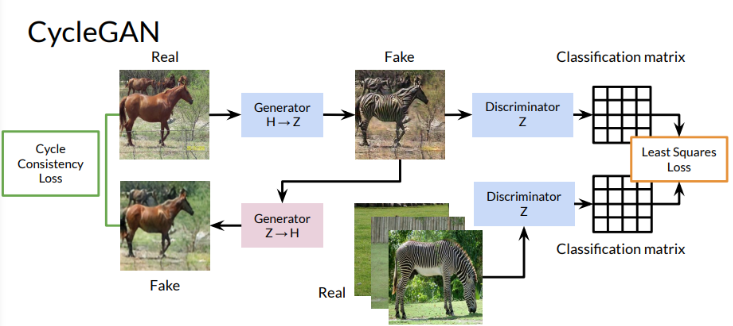
\includegraphics[scale=0.80]{Снимок.PNG}
        \end{tabular}
    \end{center}

    Мы рассмотрим более простой случай \textbf{Pix2Pix}, где есть парные данные. Формально, пусть имеется пара соответствующих друг другу картинок из двух распределений:
    \[
    x_s \sim p_s(x), \,\, x_t \sim p_t(x) \Longrightarrow \text{хотим } G(x_s) \approx x_t
    \]
    
    Для этого можно взять обычный попиксельный MSE Loss:
    \[
    \mathbb{E}_{x_s, \, x_t} \bigg[\big|\big| G(x_s) - x_t \big|\big|^2_2\bigg]
    \]
    
    Однако обучая только на него, картинки будут получаться очень размытыми, так как MSE предполагает нормальность распределения пикселей, что в реально не так.

    \pagebreak

    Поэтому дополнительно добавляется еще и GAN Loss, который вводится именно для повышения реалистичности генерации, а не проверки соответствия пар картинок друг другу. \\

    Объединяя эти два подхода, получаем составной лосс для обучения:
    \[
    \mathcal{L} = \alpha \, \text{MSE} + (1 - \alpha) \,\mathcal{L}_{GAN}(G, \, D) \longrightarrow \min_{G, \,D}, \quad \alpha \in [0, \, 1]
    \]

    \Subsection{Теоретические обоснование}\\
    
    Попробуем понять, что на самом деле происходит при оптимиации GAN лосса. Вспомним, что генератор получает $z \sim \mathcal{N}(0, \, I)$; для удобства обзовем распределение его выходов как
    \[
    x = G(z) \Longrightarrow x \sim p_{gen}(x)
    \]
    
    \underline{Зафиксируем} генератор, тогда GAN лосс принимает вид:
    \[
    \mathcal{L}_{GAN}(D) = \mathbb{E}_{\, x \sim p_{\textcolor{red}{data}}} \bigg[\log D(x)\bigg] + \mathbb{E}_{\, x \sim p_{\textcolor{red}{gen}}} \bigg[\log \left(1 - D(x)\right)\bigg] \longrightarrow \max_{D(x)}
    \]
    
    Найдем оптимальный дискриминатор $D^*(x):$
    \[
    \mathcal{L}_{GAN}(D) = \int_{x \in \mathcal{X}} \bigg[p_{data}(x) \, \log D(x) + p_{gen}(x) \, \log \left(1 - D(x)\right)\bigg]dx \longrightarrow \max_{D(x)}
    \]

    Как это максимизировать по всему пространству картинок $\mathcal{X}$ не очень понятно. Упростим нашу задачу и будем максимизировать функцию под интегралом в каждой точке:
    \[
    c := D(x) \Longrightarrow g(c) = p_{data}(x) \log c + p_{gen}(x) + \log (1 - c) \longrightarrow \max_{c}
    \]
    \[
    g'(c) = \frac{p_{data}(x)}{c} - \frac{p_{gen}(x)}{1-c} = 0 \Longrightarrow (1-c) \, p_{data}(x) - c \, p_{gen}(x) = 0
    \]
    
    Отсюда получаем оптимальный дискриминатор:
    \[
    D^*(x) = c^* = \frac{p_{data}(x)}{p_{data}(x) + p_{gen}(x)}
    \]

    Действительно, если генератор идеально обучился, то дискриминатор не сможет отличать реальные картинки от сгенерированных, а значит 
    \[
    p_{data}(x) = p_{gen}(x) \Longrightarrow D^*(x) = \frac{p_{data}(x)}{p_{data}(x) + p_{gen}(x)} = \frac{1}{2}
    \]

    \pagebreak

    Теперь подставим оптимальный дискриминатор в лосс:
    \[
    \mathcal{L}_{GAN}(D^*) = \int_{x \in \mathcal{X}} \bigg[p_{data}(x) \, \log \frac{p_{data}(x)}{p_{data}(x) + p_{gen}(x)} + p_{gen}(x) \, \log \frac{p_{gen}(x)}{p_{data}(x) + p_{gen}(x)}\bigg]dx = (*)
    \]

    Выражения очень похожие на KL-дивергенцию, но для этого нам нужно отнормировать удвоенную плотность. Прибавим и вычтем под интеграом $p_{data}(x)\log2 $ и $p_{gen}(x)\log 2:$
    \[
    (*) =  \int_{x \in \mathcal{X}} \bigg[p_{data}(x) \, \log \frac{\textcolor{blue}{2} \, \textcolor{red}{p_{data}(x)}}{\textcolor{blue}{p_{data}(x) + p_{gen}(x)}} + p_{gen}(x) \, \log \frac{\textcolor{blue}{2} \, \textcolor{red}{p_{gen}(x)}}{\textcolor{blue}{p_{data}(x) + p_{gen}(x)}}\bigg]dx -
    \]
    \[
    - \log2 \int_{x \in \mathcal{X}} \bigg[p_{data}(x) + p_{gen}(x)\bigg] \, dx = \text{KL}\left(p_{data} \,\, \bigg|\bigg| \,\,\frac{p_{data} + p_{gen}}{2}\right) + \text{KL}\left(p_{gen} \,\, \bigg|\bigg| \,\,\frac{p_{data} + p_{gen}}{2}\right) - 2\log 2 = 
    \]

    \[
    = 2 \, JS(p_{data}, \, p_{gen}) - 2\log 2
    \]

    \begin{center}
    \fbox{\begin{minipage}{0,50\textwidth}
    \[
    \textbf{Дивергенция Йенсена—Шеннона}
    \]
    \[
    JS(p \,\, \big|\big| \,\, q) = \frac{1}{2} \, \text{KL}(p \,\, \big|\big| \,\, q) + \frac{1}{2} \, (q \,\, \big|\big| \,\, p)
    \]
    \end{minipage}} 
    \end{center}

    Дивергенция Йенсена—Шеннона все еще не является метрикой, так как для нее не выполняется неравенство треугольника. Зато по сравнению с KL она симметрична и ограничена. \\

    Можно сделать вывод, что при обучении GAN минимизируется JS-дивергенция между распределением данных и генератора. На самом деле это не совсем так, потому что в реальности мы никогда не получим идеальный дискриминатор. \\
    
    Более того, если переобучить дискриминатор, то возникнет проблема затухания градиентов, при которой генератор перестанет учиться. То есть оптимальный генератор с точки зрения практики, наоборот, все ломает.

    \Subsection{Mode collapse}

    Слабым местом GANов является \textbf{mode collapse} -- свойство модели покрывать лишь очень небольшое количество мод. Иначе говоря, несмотря на то, что GANы генерируют супер реалистичные картинки, разнообразие семплов будет сильно ограничено. Решение этой проблемы не придумали, поэтому если mode collapse критичен, придется использовать другие модели.

    \begin{center}
        \begin{tabular}{cc}
            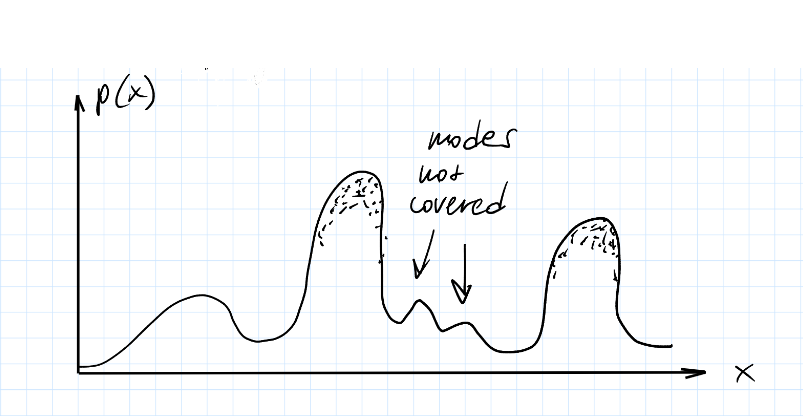
\includegraphics[scale=0.55]{Снимок2.PNG}
        \end{tabular}
    \end{center}

    
    

\end{document}
